\begin{slikaDesno}{fig/zIQ.pdf}
\PID На слици је приказан дискретан систем у коме 
су употребљени идеални множачи, и 
нископропусни каузални филтри 
\vspace*{1mm}
чија је функција преноса 
$H(\jj\Omega) = \dfrac{1 - \upalpha}{1 - 
\upalpha\ee^{-\jj\Omega}}$, где је $\upalpha = 0,8$.
Улазни сигнал је 
$x[n] = X_{\rm m} \cos(\Upomega_0 n + \upphi)$, где су 
$X_{\rm m} = 1$, 
$\Omega_0 = \dfrac{\uppi}{3}$, и $\upphi = \dfrac{\uppi}{6}$. 
\end{slikaDesno}
\begin{enumerate}[label=(\alph*)]
    \item Одредити Фуријеову 
    трансформацију побудног 
    сигнала $X(\jj\Omega) = \mathcal{FT}\{x(t)\}$,
    и скицирати његов амплитудски спектар на 
    интервалу $0 < \Omega < 2\uppi$.
    %
    \item Одредити сигнале $x_{\rm s}[n]$ и 
    $x_{\rm c}[n]$ у временском домену. 
    \item Oдредити сигнале $y_{\rm c}[n]$ и
    $y_{\rm s}[n]$ у временском домену.
    \item  На улаз система доводи 
    се сигнал истог облика, са непознатим 
    вредностима параметара $X_{\rm m}$ и $\upphi$.  
    Уколико се сматра да су употребљени филтри 
    довољно добри да у њиховом устаљеном одзиву 
    практично преостају само познате 
    једносмерне компоненте,
    $y_{\rm c}[n] \approx Y_{\rm c}$ и
    $y_{\rm s}[n] \approx Y_{\rm s}$, 
    изразити парамтре $A$ и $\upphi$ на основу 
    тих компоненти.
\end{enumerate}

\RESENJE 
На основу табличне трансформације \reft{T:DTFT:cos} је за одговарајуће вредности параметара, 
основни период на симетричном опсегу учесатности $-\uppi < \Omega < \uppi$ дат изразом
\begin{equation}
   X(\jj\Omega) = \uppi X_{\rm m} \left(
    \ee^{\jj\uppi/6} \updelta\left(\Omega - \dfrac{\uppi}{3}\right)
    +
    \ee^{-\jj\uppi/6} \updelta\left(\Omega + \dfrac{\uppi}{3}\right)
   \right). \qquad\qquad (-\uppi < \Omega < \uppi) \label{eq:\ID.xjw}
\end{equation}
Да би се одредио спектар у траженом опсегу, $0 < \Omega < 2\uppi$, потребно је 
Дираков импулс за $\Omega = -\dfrac{\uppi}{3}$ пресликати на учестаност 
$\Omega = -\dfrac{\uppi}{3} + 2\uppi = \dfrac{5\uppi}{3}$, чиме се добија 
\begin{equation}
    X(\jj\Omega) = \uppi\left(
        \ee^{\jj\uppi/6} \updelta\left(\Omega - \dfrac{\uppi}{3}\right)
        +
        \ee^{-\jj\uppi/6} \updelta\left(\Omega - \dfrac{5\uppi}{3}\right)
       \right).
\end{equation}
Амплитудски спектар, приказан на слици \ref{fig:\ID.1},
добија се одређивањем модула дате трансформације као 
\begin{eqnarray}
    |X(\jj\Omega)| = 
        \uppi 
        \updelta\left(\Omega - \dfrac{\uppi}{3}\right)
        +
        \uppi 
        \updelta\left(\Omega - \dfrac{5\uppi}{3}\right).
\end{eqnarray}

\begin{figure}[ht!]
    \centering
    \includegraphics{fig/dirac_plot.pdf}
    \caption{Тражени амплитудски спектар}
    \label{fig:\ID.1}
\end{figure}

(б) \textbf{I начин} 
Утицај датог множача може се одредити применом одгвоварајућих тригонометријских 
идентитета\footnote{Тригонометријски идентитети који се користе су 
$\cos(x)\cos(y) = \dfrac{1}{2}\bigl(
\cos(x+y) + \cos(x-y)
\bigr)$;\quad
$\cos(x)\sin(y) = \dfrac{1}{2}\bigl(
\sin(x+y) - \sin(x-y)
\bigr)$} за развој датих сигнала,
\begin{eqnarray}
    x_{\rm c}[n] &=& x[n] \cdot \cos(\Omega_0 n) 
    = X_{\rm m} \cos(\Upomega_0 n + \upphi)  \cdot \cos(\Omega_0 n)
    \\
    &=& \dfrac{X_{\rm m}}{2} \bigl( \cos(\upphi) +  \cos(2\Omega_0 n + \upphi) \bigr),
    \label{eq:\ID.rez}
\end{eqnarray}
односно
\begin{eqnarray}
    x_{\rm s}[n] &=& x[n] \cdot \sin(\Omega_0 n) 
    = X_{\rm m} \cos(\Upomega_0 n + \upphi)  \cdot \sin(\Omega_0 n)
    \\
    &=& \dfrac{X_{\rm m}}{2} \bigl( -\sin(\upphi) + \sin(2\Omega_0 n + \upphi) \bigr),
\end{eqnarray}

\textbf{II начин} Може се искористити својство о утицају Фуријеове трансформације дискретног сигнала на 
производ сигнала, као што је дато у додатку \ref{a:svojstva}, 
$\FT{x[n]\cdot y[n]} = \dfrac{1}{2\uppi} \FT{x[n]} \circledast \FT{y[n]}$. Спектар $X(\jj\Omega)$ дат је изразом 
\eqref{eq:\ID.xjw}, а спектри сигнала са којима се он множи су таблични
\begin{eqnarray}
    \FT{\cos(\Omega_0 n)} = \uppi( \updelta(\Omega - \Omega_0)  +  \updelta(\Omega + \Omega_0)  )     \\
    \FT{\sin(\Omega_0 n)} = \uppi( \updelta(\Omega - \Omega_0)  -  \updelta(\Omega + \Omega_0)  )     
    \label{eq:\ID.sincos}
\end{eqnarray}

\begin{figure}[ht!]
    \centering
    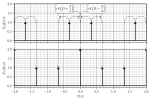
\includegraphics{fig/conv_delta_ilustration.pdf}
    \caption{Уз објашњење кружне конволуције}
    \label{fig:\ID.circconv}
\end{figure}

Поступак ће бити детаљно описан и илустрован за случај за множење са сигналом $\cos(\Omega_0 n)$. 
Кружна конволуција два периодична сигнала рачуна се одређивањем конволуције једног са периодичном основом другог
(видети и додатак \ref{a:svojstva}). У овом случају,
за периодичну основу могу се узети по два Диракова импулса у интервалу $-\uppi < \Omega < \uppi$ из израза
\eqref{eq:\ID.sincos}. Пошто коволуција са $\updelta(\Omega \pm \Omega_0)$ представља транслацију сигнала 
у учестности за $\Omega_0$, то ова операција представља сабирање две транслиране поворке, једне у десно за 
$\Omega_0$ и друге лево за $\Omega_0$. Овај процес илустрован је на слици 
\ref{fig:\ID.circconv}. Приметимо да се сваки од импулса помера за $\Omega_0$, а да се нарочито импулси 
на учестаношћу $\pm \Omega_0$ сабирају до импулса у нули (односно на DC). Одговарајућим 
Сабирањем два најближа импулса око нуле добија се 
\begin{equation}
    \underbrace{\dfrac{1}{2\uppi}}_{\mathclap{\text{Коефицијент из особине}}}
    \overbrace{
    \left[
        \uppi X_{\rm m}
        \ee^{\jj\upphi} \updelta\left(\Omega\right)
        +
        \uppi X_{\rm m}
        \ee^{-\jj\upphi} \updelta\left(\Omega\right)
    \right]}^{
        \mathclap{\text{Одговарајуће померени импулси $X(\jj\Omega)$.}}
    }
    \underbrace{\uppi}_{\mathclap{\text{Коефицијент испред импулса у спектру косинуса}}}
    =
    \uppi X_{\rm m} \cos (\upphi) \updelta(\Omega).
\end{equation}
Добијени резултат представља Дираков импулс у нули, а због периодичности спектра и Дираков импулс на свим 
$\Omega = 2k\uppi$, $k \in \mathbb Z$. Услед табличне трансформације 
\reft{T:DTFT:const}, овај члан онда одговара константи $X_{\rm m} \cos(\upphi)/2$. 

Преостале конволуције појединачних импулса су непреклапајуће 
па се добијају остали импулси на релевантном интервалу
\begin{equation}
    \uppi \dfrac{X_{\rm m}}{2} ( \ee^{\jj\upphi} \updelta(\Omega - 2\Omega_0) + \ee^{-\jj\upphi} \updelta(\Omega + 2\Omega_0)  ),
\end{equation}
што таблично одговара сигналу $\dfrac{X_{\rm m}}{2} \cos(2\Omega_0 n + \upphi)$. Сабирањем добијене константне 
вредности и синусоиде добија се исти резултат као и \eqref{eq:\ID.rez}. Поступак за синусни сигнал је потпуно 
аналоган и препоручује се за вежбу. 

(в) Филтар се побуђује на учестностима $\Omega = 2\Omega_0$ и $\Omega = 0$, па се прво може израчунати 
ампитудско појачање и фазни померај на ове две учестаности,
\begin{eqnarray}
    H(0) &=& \dfrac{1 - \upalpha}{1 - \upalpha \ee^{-\jj 0}} = 1; \text{ и} \\ 
    H(\jj 2\Omega_0) &=& \dfrac{1 - \upalpha}{1 - \upalpha \ee^{-\jj2\Omega_0}} = 
    \dfrac{1}{\sqrt{21}} \, \ee^{-\jj\arctan\left(2/\sqrt 3\right)} \approx 
    0,21 \ee^{-\jj\,0,85}.
\end{eqnarray}
Пошто филтре побуђују само простопериодични сигнали, због линеарности су 
\begin{eqnarray}
    y_{\rm c}[n] 
    &=&
    \dfrac{X_{\rm m}}{2} \biggl( |H(0)| \cos(\upphi) 
    + |H(\jj 2 \Omega_0)| \cos \bigl(2\Omega_0 n + \upphi + \arg\,H(\jj2\Omega_0) \bigr) \biggr), \\
    &=&
    \dfrac{X_{\rm m}}{2} 
    \left(
        \cos(\upphi) + \dfrac{1}{\sqrt{21}} 
        \cos(2\Omega_0 n + \upphi -\arctan( {2}/{\sqrt 3}) )
    \right) \\
    &=& 
    \dfrac{\sqrt 3}{4} 
    + 
    0,11 \cos\left( \dfrac{2\uppi n}{3} - 0,33  \right),
\end{eqnarray}
и потпуно аналогно за синусну грану
\begin{eqnarray}
    y_{\rm s}[n] &=& 
    \dfrac{X_{\rm m}}{2} 
    \left(
        -\sin(\upphi) + \dfrac{1}{\sqrt{21}} 
        \sin(2\Omega_0 n + \upphi -\arctan( {2}/{\sqrt 3}) )
    \right) \\
    &=&
    -\dfrac{1}{4} 
    + 0,11 \sin\left( \dfrac{2\uppi n}{3} - 0,33  \right),
\end{eqnarray}

\begin{wrapfigure}{r}{0.3\textwidth}
    
\includegraphics{fig/zIQ_resenje.pdf}
    \caption{Уз тачку (г).}
    \label{fig:\ID.uzg}
\end{wrapfigure}
(г) По претпоставци задатка, компоненте сигнала које остају након филтрирања су  
само сталне вредности, и то 
$Y_{\rm c} = \dfrac{X_{\rm m}}{2}\cos(\upphi)$ и 
$Y_{\rm s} = -\dfrac{X_{\rm m}}{2}\sin(\upphi)$. 
За решавање задатка може бити корисно уочити  да дате вредности представљају координате тачке 
на кружници полупречника $X_{\rm m}/2$ која са апсцисом заклапа угао $-\upphi$, као што је 
илустровано на слици \ref{fig:\ID.uzg}. Трансформацијом координата добијају се тражене везе, 
и то $X_{\rm m} = 2\sqrt{Y_{\rm c}^2 + Y_{\rm s}^2}$ и 
$\upphi = -\arctan\left(Y_{\rm s}/Y_{\rm c}\right)$. Слични изрази се могу одредити и
третирајући комплексан број $Y = Y_{\rm c} - \jj Y_{\rm s}$, у ком случају су 
$X_{\rm m} = 2 |Y|$ и $\upphi = \arg Y$. 

